\begin{frame}{Problem Definition}
Given two strings text1 and text2, return the length of their longest common subsequence
\end{frame}

\begin{frame}[label=conclusion, standout]
    \begin{center}
    \LARGE What is a sub-sequence?
    \end{center}
\end{frame}

\begin{frame}{Subsequence}
A sub-sequence is a sequence that can be obtained by deleting elements from the original sequence without changing order of the elements.
\pause

Let str = "ABCDE" be a sequence

\begin{center}
    
\begin{adjustbox}{max totalsize={\textwidth}{0.5\textheight}}
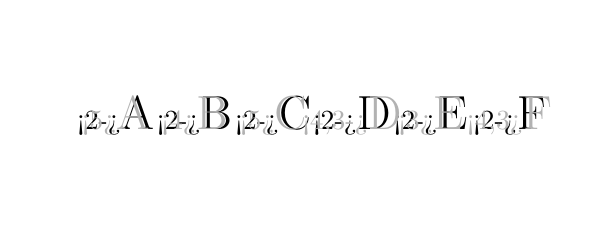
\begin{tikzpicture}

    \node at (0,0) {};
    \node at (2,2) {};
    
    \node[rectangle] at (1,1) {{\onslide<2->{\LARGE{A}}}};
    \node[rectangle] at (2,1) {{\onslide<2->{\LARGE{B}}}};
    \node[rectangle] at (3,1) {{\onslide<2->{\LARGE{C}}}};
    \node[rectangle] at (4,1) {{\onslide<2->{\LARGE{D}}}};
    \node[rectangle] at (5,1) {{\onslide<2->{\LARGE{E}}}};
    \node[rectangle] at (6,1) {{\onslide<2->{\LARGE{F}}}};

    \node[rectangle, text = gray!60] at (1,1) {{\onslide<5>{\LARGE{A}}}};
    \node[rectangle, text = gray!60] at (2,1) {{\onslide<4>{\LARGE{B}}}};
    \node[rectangle, text = gray!60] at (3,1) {{\onslide<5>{\LARGE{C}}}};
    \node[rectangle, text = gray!60] at (4,1) {{\onslide<4,3->{\LARGE{D}}}};
    \node[rectangle, text = gray!60] at (5,1) {{\onslide<3>{\LARGE{E}}}};
    \node[rectangle, text = gray!60] at (6,1) {{\onslide<4,3>{\LARGE{F}}}};
    
\end{tikzpicture}
\end{adjustbox}
\end{center}
\onslide<3->{Then some subsequnce of str are : \quad ABC \onslide<4->{\quad ACE \quad \onslide<5->{BEF \quad etc.}}}

\end{frame}







